\section{Diagrammes de séquences}
Le diagramme de séquence représente l’interaction des acteurs avec notre système selon un
enchaînement chronologique. Ceci dit, que la représentation des cas de figures par des diagrammes
de séquence va nous permettre de schématiser la collaboration entre les objets du système d’un point
de vue temporel.\\
Dans ce qui suit, on va présenter les diagrammes de séquences relatives à quelques cas d'utilisation.

\subsection{Diagramme de séquence « s’authentifier »}
Le cas d’utilisation « s’authentifier » se déclenche une fois l’utilisateur tente d’accéder à l'application.\newpage
\newpage
\begin{table}[!h]
\begin{tabular}{|p{15cm}|}%p{2.5cm}|p{9cm}
\rowcolor{shadecolor}\multicolumn{1}{|c|}{Description des scénarios} \\
\hline
\textbf{Scénario nominal :}
\begin{itemize}[label=\textbullet]
  \item l'utilisateur saisie le nom d'utilisateur et le mot de passe
  \item le système vérifie la validité du nom d'utilisateur et le mot de passe
  \item si l'authentification est réussite, l'utilisateur sera redirigé vers la page d'accueil, sinon un message d'erreur sera affiché
\end{itemize}
	\\
\hline
\end{tabular}
\end{table}
\begin{figure}[h!]  
 \centering
    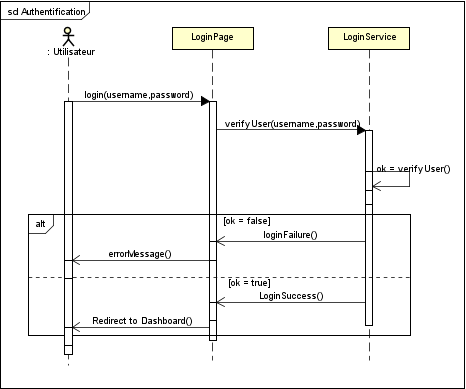
\includegraphics{chapitre4/Figures/authentification.png}
  \caption{Diagramme de séquence du cas d'utilisation « S’authentifier »}
\end{figure}

\subsection{Diagramme de séquence « Mot de passe oublié »}
La figure suivante présente le diagramme de séquence du scénario " Mot de passe oublié" mettant en évidence l’ensemble des interactions entre l'utilisateur d’une part et l’ensemble des composants du système d’une autre part.\newpage
\newpage
\begin{table}[!h]
\begin{tabular}{|p{15cm}|}%p{2.5cm}|p{9cm}
\rowcolor{shadecolor}\multicolumn{1}{|c|}{Description des scénarios} \\
\hline
\textbf{Scénario nominal :}
\begin{itemize}[label=\textbullet]
  \item l'utilisateur saisie son nom d'utilisateur
  \item le système vérifie la validité du nom d'utilisateur
  \item si le nom d'utilisateur est valide, le système enverra un mail à l'utilisateur et affichera un message de succès, sinon, un message d'erreur sera affiché
\end{itemize}
	\\
\hline
\end{tabular}
\end{table}
\begin{figure}[h!]  
 \centering
    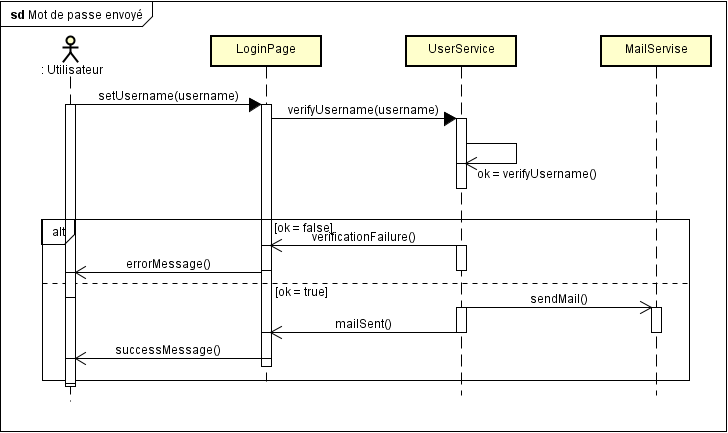
\includegraphics[width=0.9\textwidth]{chapitre4/Figures/mdpoublie.png}
  \caption{Diagramme de séquence du cas d'utilisation « Mot de passe oublié »}
\end{figure}

\subsection{Diagramme de séquence « Gestion des régions »}
La figure suivante présente le diagramme de séquence du scénario "Gestion des régions" mettant en évidence l’ensemble des interactions entre l'administrateur d’une part et l’ensemble des composants du système d’une autre part. Ce scénario permet l'ajout, la modification et la suppression d'une région.
\newpage
\begin{table}[!h]
\begin{tabular}{|p{15cm}|}%p{2.5cm}|p{9cm}
\rowcolor{shadecolor}\multicolumn{1}{|c|}{Description des scénarios} \\
\hline
\textbf{Scénario nominal :}
\begin{itemize}
\item Ajouter région
\begin{itemize}[label=\textbullet]
  \item l'utilisateur saisie le formulaire pour ajouter une région
  \item le système vérifie la validité des données saisies, s'ils sont valides, il ajoutera une nouvelle région, sinon un message d'erreur sera affiché
\end{itemize}
\item Modifier région
\begin{itemize}[label=\textbullet]
  \item l'utilisateur choisiras une région à modifier
  \item l'utilisateur saisie les modifications souhaités
  \item le système vérifie la validité des données saisies, s'ils sont valides, il modifiera une nouvelle région, sinon un message d'erreur sera affiché
\end{itemize}
\item Supprimer région
\begin{itemize}[label=\textbullet]
  \item l'utilisateur choisiras une région à supprimer
  \item le système affichera un message de confirmation et attendra l'utilisateur pour valider la suppression
  \item une fois validé, le système supprimera la région de la base de données 
\end{itemize}
\end{itemize}
	\\
\hline
\end{tabular}
\end{table}
\begin{figure}[h!]  
 \centering
    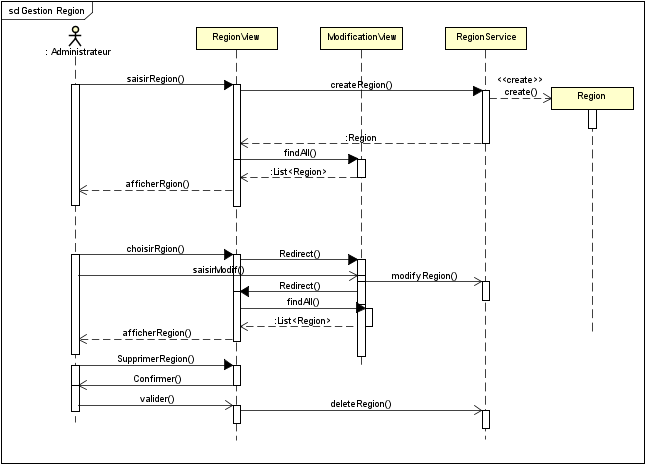
\includegraphics[width=0.92\textwidth]{chapitre4/Figures/region.png}
  \caption{Diagramme de séquence du cas d'utilisation « Gestion des régions »}
\end{figure}
\newpage
\subsection{Diagramme de séquence «Suivi des FDT »}
La figure suivante présente le diagramme de séquence du scénario "Suivi des FDT" mettant en évidence l’ensemble des interactions entre l'utilisateur d’une part et l’ensemble des composants du système d’une autre part. Ce scénario permet l'ajout, la modification, ainsi la consultation des synthèses des FDT.

\begin{table}[!h]
\begin{tabular}{|p{15cm}|}%p{2.5cm}|p{9cm}
\rowcolor{shadecolor}\multicolumn{1}{|c|}{Description des scénarios} \\
\hline
\textbf{Scénario nominal :}
\begin{itemize}[label=\textbullet]
  \item le système affiche la liste des feuilles manquantes par directeur de projet
  \item pour une date donnée et pour un directeur de projet précis, l'utilisateur saisie le nombre de feuilles de temps manquantes 
  \item l'utilisateur peut visualiser des graphes synthétisant le taux de saisie des feuilles de temps par directeur de projet
\end{itemize}
	\\
\hline
\end{tabular}
\end{table}

\begin{figure}[h!]  
 \centering
    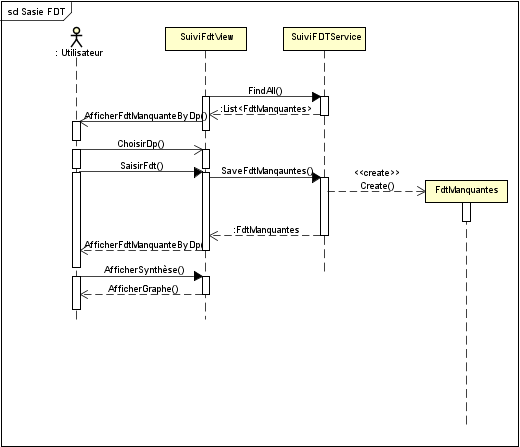
\includegraphics{chapitre4/Figures/suivifdt.png}
  \caption{Diagramme de séquence du cas d'utilisation « Suivi des FDT »}
\end{figure}